% ==================== 2.4.3 三重旋转反演轴 ====================
\subsubsection{三重旋转反演轴（\texorpdfstring{$P\,\bar3$}{P-3}）}

旋转反演轴 $\bar n$ 是一条几何直线，其操作为旋转 $2\pi/n$ 与反演 $\bar1$ 的联合操作
（先旋转、再反演）。为观察 $\bar3$ 轴，选用空间群 $P\,\bar3$（No.~147，三方晶系，
$\bar3$ 轴沿 $c$ 方向），建模参数见表~\ref{tab:sym-rotinv3}。

\begin{table}[H]
  \centering
  \caption{三重旋转反演轴演示的建模参数}
  \label{tab:sym-rotinv3}
  \begin{tabular}{ll}
    \toprule
    项目 & 参数 \\
    \midrule
    空间群 & $P\,\bar3$（No.~147，三方晶系） \\
    晶格常数 & $a=b=c=2.0$\,\AA，$\alpha=\beta=90^\circ$，$\gamma=120^\circ$ \\
    原子坐标 & Si：$(0.2,\,0.3,\,0.4)$（一般位置） \\
    等效位置数 & 6（单胞内 6 个原子） \\
    \bottomrule
  \end{tabular}
\end{table}

\begin{figure}[H]
  \centering
  \subcaptionbox{(a) 空间群与晶胞参数设置}{%
    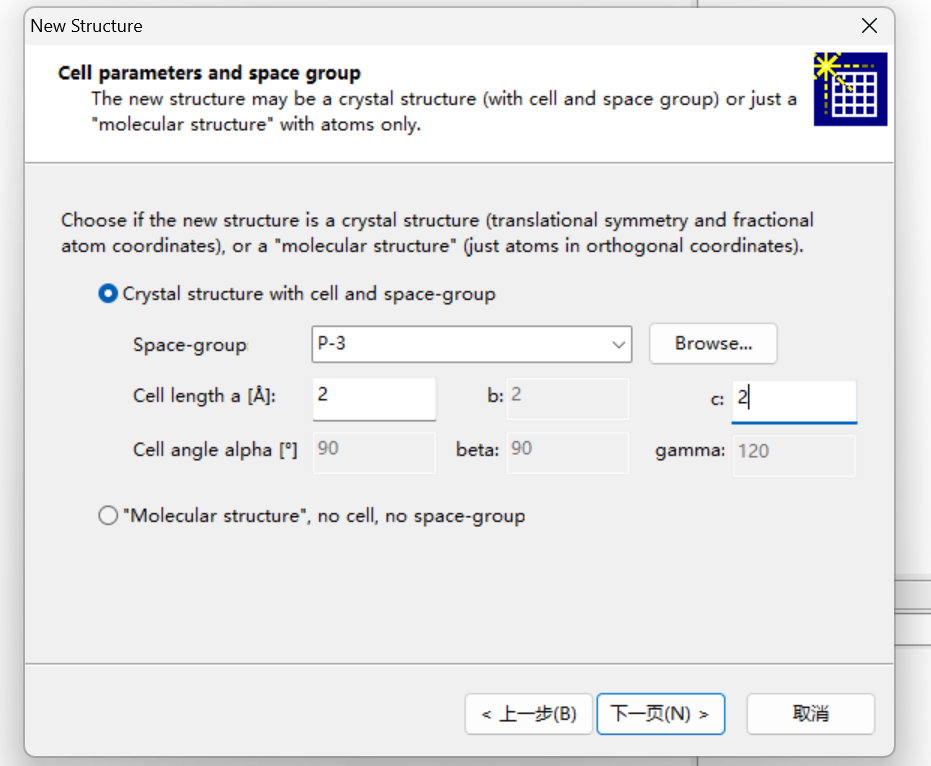
\includegraphics[width=0.44\textwidth]{assets/symmetry/rotoinversion3/a.png}}
  \hfill
  \subcaptionbox{(b) 非对称单元原子（Si）添加}{%
    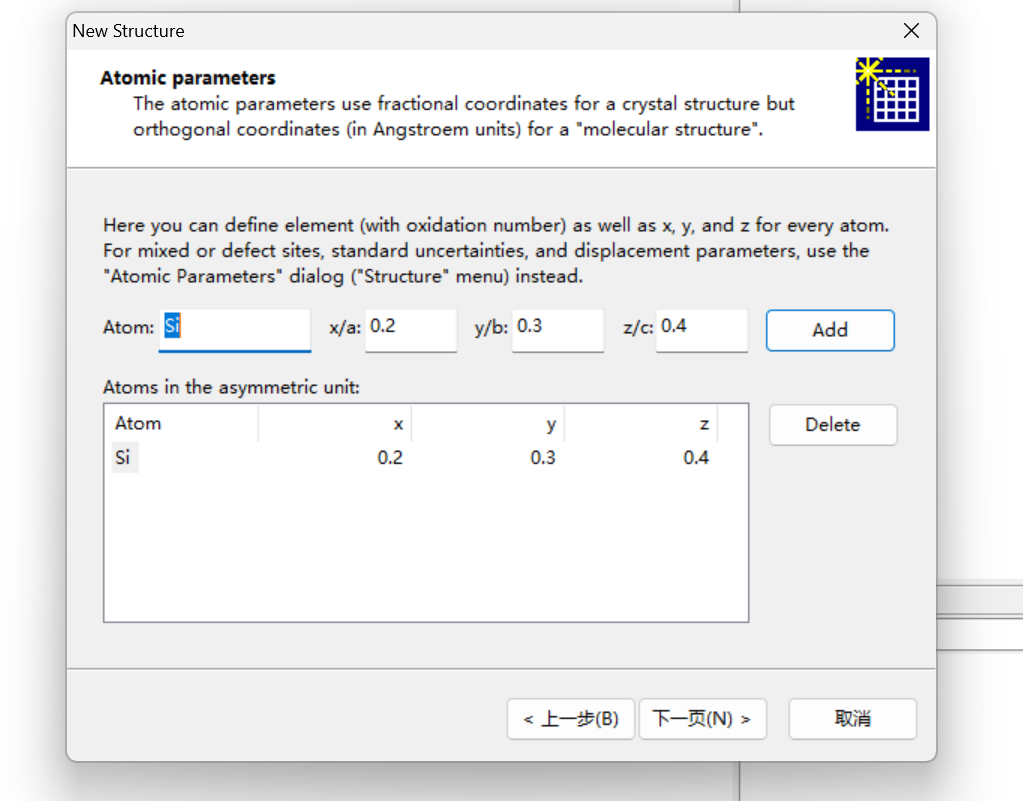
\includegraphics[width=0.44\textwidth]{assets/symmetry/rotoinversion3/b.png}}
  \caption{三重旋转反演轴（$P\,\bar3$）演示的参数设置}
  \label{fig:sym-rotinv3-param}
\end{figure}

\begin{figure}[H]
  \centering
  \subcaptionbox{(a) 单胞图：6 个原子分居上下两层（每层 3 个）}{%
    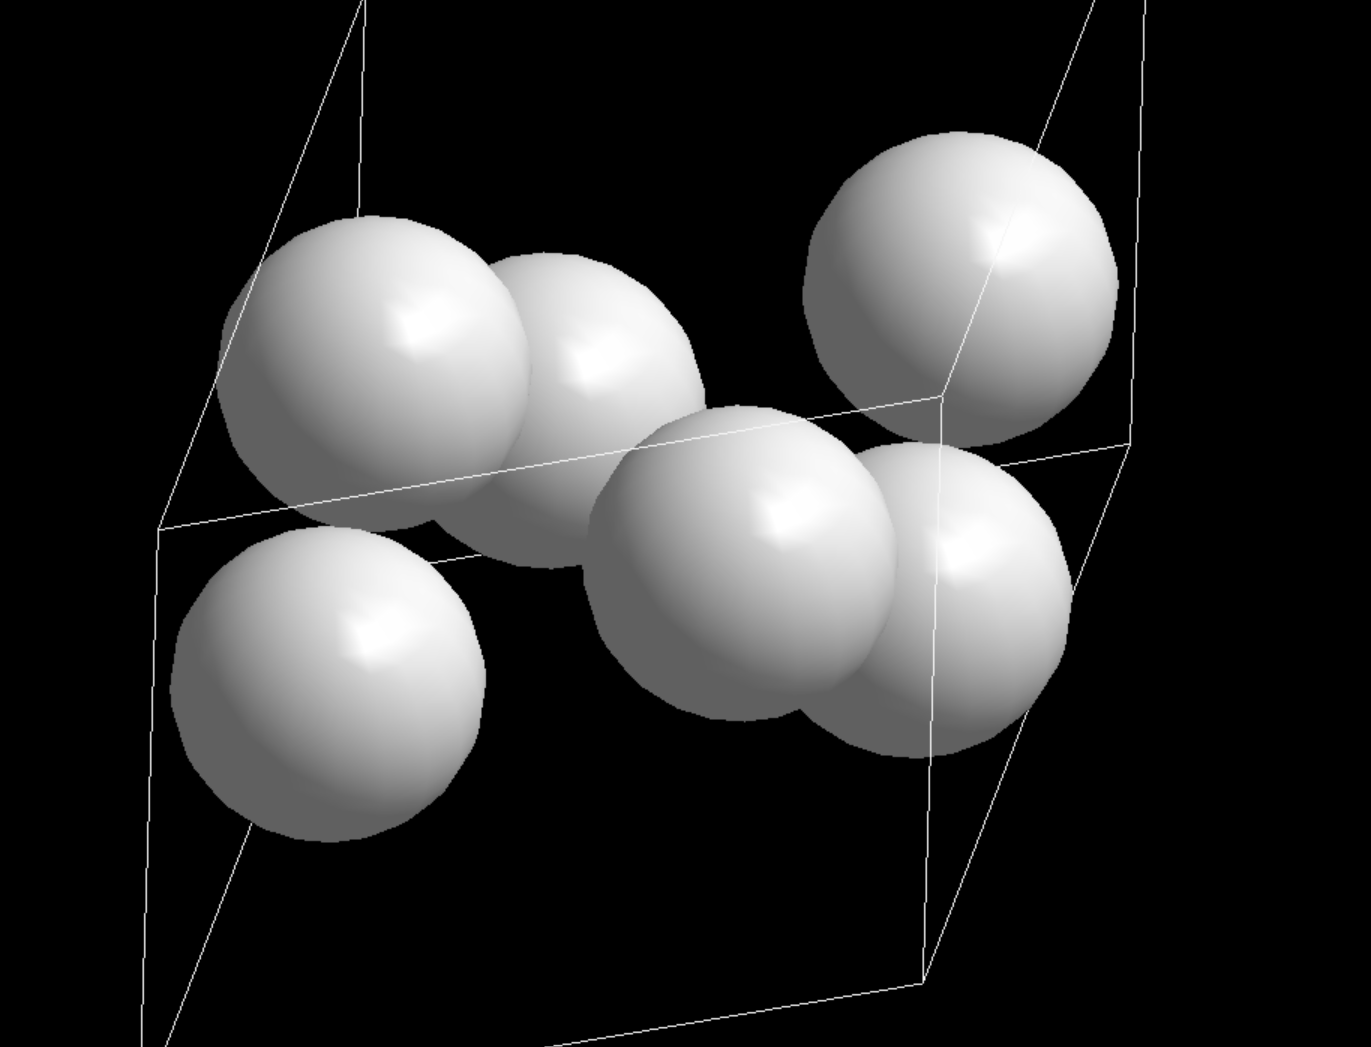
\includegraphics[width=0.44\textwidth]{assets/symmetry/rotoinversion3/c.png}}
  \hfill
  \subcaptionbox{(b) 超晶胞图：双层原子组的周期排列}{%
    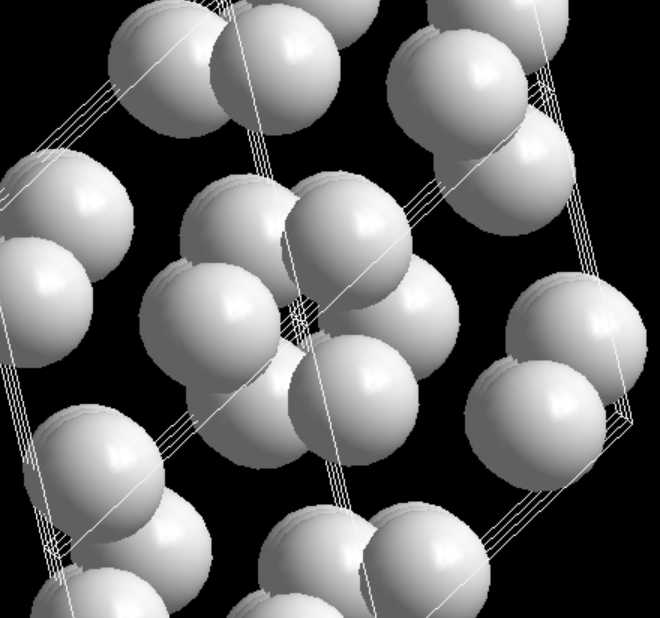
\includegraphics[width=0.44\textwidth]{assets/symmetry/rotoinversion3/d.png}}
  \caption{三重旋转反演轴（$P\,\bar3$）的单胞与超晶胞模型}
  \label{fig:sym-rotinv3-model}
\end{figure}

$P\,\bar3$ 的一般位置等效位置为
\begin{equation}
  \begin{aligned}
    \bar3:\quad &(x,y,z),\quad (\bar y,\,x-y,\,z),\quad (-x+y,\,\bar x,\,z);\\
    &(\bar x,\,\bar y,\,\bar z),\quad (y,\,-x+y,\,\bar z),\quad (x-y,\,x,\,\bar z)
  \end{aligned}
\end{equation}
上半行是绕 $c$ 轴旋转 $120^\circ$ 得到的 3 个原子（$z$ 不变），下半行是它们逐一反演
得到的 3 个原子。将 Si 的坐标 $(0.2,0.3,0.4)$ 代入，6 个原子的分数坐标为
$(0.2,0.3,0.4)$、$(0.7,0.9,0.4)$、$(0.1,0.8,0.4)$（上层，$z=0.4$）与
$(0.8,0.7,0.6)$、$(0.3,0.1,0.6)$、$(0.9,0.2,0.6)$（下层，$z=0.6$）。可见旋转反演
操作产生的原子不位于同一平面，而是分居上下两层
（图~\ref{fig:sym-rotinv3-model}(a)）；超晶胞中双层原子组沿空间周期排列
（图~\ref{fig:sym-rotinv3-model}(b)）。因此，$\bar3$ 等效于 $3+\bar1$ 的联合：先经
3 次轴旋转得到 3 个原子，再经反演得到另外 3 个原子。

\textbf{特征与辨识要点。}$\bar3$ 的完整联合操作需依次进行 6 次才能回到初始位置，
故单胞内出现 6 个（而不是 3 个）等效原子——操作次数为 6 而非 3，这是旋转反演轴的
特有性质。若从平行于 $\bar3$ 轴的方向观察，6 个原子看似呈六重对称分布，容易与
6 次旋转轴混淆；两者的区别在于：旋转反演产生的原子分居上下两层、两层之间存在
反演对应关系，而 6 次旋转轴产生的 6 个原子位于垂直轴的同一平面内。$\bar3$ 是
立方晶系沿体对角线方向的特征对称元素（如 $F\,m\,\bar3\,m$ 中的 $\bar3$）。
